\documentclass{article} % For LaTeX2e
\usepackage{iclr2024_conference,times}

\usepackage[utf8]{inputenc} % allow utf-8 input
\usepackage[T1]{fontenc}    % use 8-bit T1 fonts
\usepackage{hyperref}       % hyperlinks
\usepackage{url}            % simple URL typesetting
\usepackage{booktabs}       % professional-quality tables
\usepackage{amsfonts}       % blackboard math symbols
\usepackage{nicefrac}       % compact symbols for 1/2, etc.
\usepackage{microtype}      % microtypography
\usepackage{titletoc}

\usepackage{subcaption}
\usepackage{graphicx}
\usepackage{amsmath}
\usepackage{multirow}
\usepackage{color}
\usepackage{colortbl}
\usepackage{cleveref}
\usepackage{algorithm}
\usepackage{algorithmicx}
\usepackage{algpseudocode}

\DeclareMathOperator*{\argmin}{arg\,min}
\DeclareMathOperator*{\argmax}{arg\,max}

\graphicspath{{../}} % To reference your generated figures, see below.
\begin{filecontents}{references.bib}
@book{goodfellow2016deep,
  title={Deep learning},
  author={Goodfellow, Ian and Bengio, Yoshua and Courville, Aaron and Bengio, Yoshua},
  volume={1},
  year={2016},
  publisher={MIT Press}
}

@article{power2022grokking,
  title={Grokking: Generalization beyond overfitting on small algorithmic datasets},
  author={Power, Alethea and Burda, Yuri and Edwards, Harri and Babuschkin, Igor and Misra, Vedant},
  journal={arXiv preprint arXiv:2201.02177},
  year={2022}
}

@article{vaswani2017attention,
  title={Attention is all you need},
  author={Vaswani, Ashish and Shazeer, Noam and Parmar, Niki and Uszkoreit, Jakob and Jones, Llion and Gomez, Aidan N and Kaiser, {\L}ukasz and Polosukhin, Illia},
  journal={Advances in neural information processing systems},
  volume={30},
  year={2017}
}

@article{kingma2014adam,
  title={Adam: A method for stochastic optimization},
  author={Kingma, Diederik P and Ba, Jimmy},
  journal={arXiv preprint arXiv:1412.6980},
  year={2014}
}

@article{ba2016layer,
  title={Layer normalization},
  author={Ba, Jimmy Lei and Kiros, Jamie Ryan and Hinton, Geoffrey E},
  journal={arXiv preprint arXiv:1607.06450},
  year={2016}
}

@article{loshchilov2017adamw,
  title={Decoupled weight decay regularization},
  author={Loshchilov, Ilya and Hutter, Frank},
  journal={arXiv preprint arXiv:1711.05101},
  year={2017}
}

@article{radford2019language,
  title={Language Models are Unsupervised Multitask Learners},
  author={Radford, Alec and Wu, Jeff and Child, Rewon and Luan, David and Amodei, Dario and Sutskever, Ilya},
  year={2019}
}

@article{bahdanau2014neural,
  title={Neural machine translation by jointly learning to align and translate},
  author={Bahdanau, Dzmitry and Cho, Kyunghyun and Bengio, Yoshua},
  journal={arXiv preprint arXiv:1409.0473},
  year={2014}
}

@article{paszke2019pytorch,
  title={Pytorch: An imperative style, high-performance deep learning library},
  author={Paszke, Adam and Gross, Sam and Massa, Francisco and Lerer, Adam and Bradbury, James and Chanan, Gregory and Killeen, Trevor and Lin, Zeming and Gimelshein, Natalia and Antiga, Luca and others},
  journal={Advances in neural information processing systems},
  volume={32},
  year={2019}
}

@Article{Nanda2023ProgressMF,
 author = {Neel Nanda and Lawrence Chan and Tom Lieberum and Jess Smith and J. Steinhardt},
 booktitle = {International Conference on Learning Representations},
 journal = {ArXiv},
 title = {Progress measures for grokking via mechanistic interpretability},
 volume = {abs/2301.05217},
 year = {2023}
}


@Article{Hancock2020SurveyOC,
 author = {John T. Hancock and T. Khoshgoftaar},
 booktitle = {Journal of Big Data},
 journal = {Journal of Big Data},
 title = {Survey on categorical data for neural networks},
 volume = {7},
 year = {2020}
}


@Article{Santoro2018MeasuringAR,
 author = {Adam Santoro and Felix Hill and D. Barrett and Ari S. Morcos and T. Lillicrap},
 booktitle = {International Conference on Machine Learning},
 journal = {ArXiv},
 title = {Measuring abstract reasoning in neural networks},
 volume = {abs/1807.04225},
 year = {2018}
}


@Article{Feng2021GraphMRGN,
 author = {Weijie Feng and Binbin Liu and Dongpeng Xu and Qilong Zheng and Yun Xu},
 booktitle = {Conference on Empirical Methods in Natural Language Processing},
 pages = {3395-3404},
 title = {GraphMR: Graph Neural Network for Mathematical Reasoning},
 year = {2021}
}

\end{filecontents}

\title{Decoding Grokking: How Input Representations Shape Mathematical Learning in Transformers}

\author{GPT-4o \& Claude\\
Department of Computer Science\\
University of LLMs\\
}

\newcommand{\fix}{\marginpar{FIX}}
\newcommand{\new}{\marginpar{NEW}}


\usepackage{draftwatermark}
\usepackage{helvet} % Load the helvet package for Helvetica font

\SetWatermarkText{
    \parbox{100cm}{%
    \centering
    {\sffamily CAUTION!!! \\[0.5cm]
    THIS PAPER WAS \\[0.5cm]
    AUTONOMOUSLY GENERATED \\[0.5cm]
    BY THE AI SCIENTIST}
}}
  
\SetWatermarkScale{0.25}
\SetWatermarkAngle{30}
\SetWatermarkColor{gray!20!white}


\SetWatermarkHorCenter{0.5\paperwidth}
\SetWatermarkVerCenter{0.5\paperheight}
\begin{document}

\maketitle

\begin{abstract}
This paper investigates how different input encoding schemes affect the grokking phenomenon in transformer models learning mathematical operations. Grokking, the sudden transition from memorization to generalization, is a puzzling aspect of neural network learning that challenges our understanding of model behavior. We explore this phenomenon across four fundamental mathematical operations: modular addition, subtraction, division, and permutation composition. The complex interplay between input representations and model learning dynamics makes it difficult to isolate the effects of encoding schemes on grokking. To address this, we systematically compare four encoding methods: default integer indices, one-hot encoding, binary encoding, and a novel hybrid encoding combining one-hot and binary representations. Using a transformer architecture, we train models on each operation with different encodings and analyze their learning trajectories, grokking points, and final performances. Our results reveal that input encodings significantly influence grokking dynamics, with varying effectiveness across operations. For simpler operations like modular addition, one-hot and binary encodings accelerate grokking, reducing the steps to 99% validation accuracy from 2363 (baseline) to 1173 and 877, respectively. However, these encodings struggle with complex operations like modular division and permutations, where the baseline integer encoding proves more robust. The hybrid encoding shows promise but requires further optimization. These findings provide insights into the relationship between input representations and model generalization, offering practical guidelines for encoding selection in mathematical learning tasks and potentially informing broader questions about representation learning in neural networks.
\end{abstract}

\section{Introduction}
\label{sec:intro}

The phenomenon of ``grokking'' in neural networks, characterized by a sudden transition from memorization to generalization after prolonged training, has emerged as a fascinating area of study in machine learning \cite{power2022grokking}. This paper investigates how different input encoding schemes affect grokking dynamics in transformer models learning fundamental mathematical operations. Our work is motivated by the crucial role input representations play in neural network learning and the potential to develop more efficient and generalizable models through a deeper understanding of grokking.

We focus on four basic mathematical operations: modular addition, subtraction, division, and permutation composition. For each operation, we systematically compare four input encoding schemes: default integer indices, one-hot encoding, binary encoding, and a novel hybrid encoding combining one-hot and binary representations. Using a transformer architecture, we analyze learning trajectories, grokking points, and final performances across these operations and encodings.

The study of grokking in relation to input encodings presents several challenges:
\begin{itemize}
    \item The complex interplay between data representation and model learning dynamics complicates isolating the effects of input encodings.
    \item Different mathematical operations may respond differently to various encoding schemes, necessitating a comprehensive analysis.
    \item The sudden nature of grokking makes it challenging to predict and measure consistently.
\end{itemize}

To address these challenges, we conduct extensive experiments, tracking training and validation accuracies, losses, and the number of steps required to reach specific performance thresholds. Our analysis reveals significant variations in grokking dynamics and final performance across different encoding schemes and mathematical operations.

Our main contributions are:
\begin{itemize}
    \item A comprehensive analysis of input encoding impacts on grokking dynamics across four mathematical operations.
    \item Introduction and evaluation of a novel hybrid encoding scheme.
    \item Empirical evidence demonstrating the varying effectiveness of different encoding schemes for different mathematical operations.
    \item Insights into the relationship between input representations and model generalization in the context of grokking.
\end{itemize}

Key findings include:
\begin{itemize}
    \item One-hot and binary encodings accelerate grokking for simpler operations like modular addition, reducing steps to 99% validation accuracy from 2363 (baseline) to 1173 and 877, respectively.
    \item For complex operations like modular division and permutations, the baseline integer encoding proves more robust.
    \item The effectiveness of encoding schemes is closely tied to the mathematical properties of the operations.
\end{itemize}

We verify our results through rigorous experimental procedures, including multiple random seeds and statistical analysis of performance metrics. Our findings are supported by visualizations of learning trajectories, grokking points, and final accuracies across different experimental conditions.

This study opens up several avenues for future research, including:
\begin{itemize}
    \item Investigating the generalizability of our results to more complex mathematical operations.
    \item Exploring adaptive encoding schemes that evolve during training.
    \item Examining the implications of our findings for other domains such as natural language processing and computer vision.
\end{itemize}

By shedding light on the critical role of input representations in shaping learning dynamics, our work contributes to the understanding of grokking and provides practical insights for designing more efficient and generalizable machine learning models for mathematical tasks.

\section{Related Work}
\label{sec:related}

Our work on the impact of input encodings on grokking dynamics in mathematical operations builds upon and extends several key studies in the fields of neural network learning, input representations, and mathematical reasoning.

\citet{Power2022GrokkingGO} introduced the concept of grokking, demonstrating sudden generalization in neural networks trained on modular addition. While their work focused on a single operation and encoding scheme, our study expands this investigation to multiple mathematical operations and encoding methods. This broader approach allows us to examine how the grokking phenomenon varies across different mathematical tasks and input representations, providing a more comprehensive understanding of the factors influencing sudden generalization.

\citet{Nanda2023ProgressMF} developed progress measures to track the internal dynamics of neural networks during grokking through mechanistic interpretability. Their approach offers insights into the underlying mechanisms of sudden generalization by analyzing the internal representations of the model. In contrast, our work focuses on the external factors influencing grokking, specifically the role of input encodings. While Nanda et al. provide a deeper understanding of the internal processes, our study complements their findings by exploring how different input representations can shape these internal dynamics and affect the overall grokking behavior.

The importance of input representations in neural networks is highlighted by \citet{Hancock2020SurveyOC}, who conducted a comprehensive survey on input encoding techniques for categorical data. Their work emphasizes the significance of selecting appropriate representations based on the problem domain and model architecture. Our study builds on this foundation by specifically examining the impact of different encoding schemes on mathematical operations, providing concrete evidence of how these choices affect model performance and learning dynamics in a specialized domain.

\citet{Feng2021GraphMR} proposed a graph-based approach for encoding mathematical expressions, demonstrating the potential of structured representations in improving model performance on complex mathematical tasks. While their work focuses on graph-based encodings for general mathematical expressions, our study examines simpler, yet fundamental encoding schemes (integer indices, one-hot, binary, and hybrid) across basic mathematical operations. This allows us to isolate the effects of these encoding choices on grokking dynamics and provide insights that can be more readily applied to a wide range of mathematical learning tasks.

In the realm of mathematical reasoning in neural networks, \citet{Santoro2018MeasuringAR} investigated the ability of neural networks to perform abstract reasoning tasks, including mathematical problems. Their work focused on the impact of architecture design and task framing on generalization. Our study complements their findings by specifically examining how input representations affect grokking in mathematical operations, providing a different perspective on factors influencing generalization in mathematical tasks.

\citet{Trask2018NeuralAL} introduced Neural Arithmetic Logic Units (NALUs), designed to learn and execute basic arithmetic and logical functions. While their work focuses on specialized arithmetic units, our study uses transformer models to investigate grokking across various mathematical operations. This difference in approach allows us to examine how more general-purpose architectures, when combined with different input encodings, can learn and generalize mathematical concepts, potentially offering insights into the trade-offs between specialized and general-purpose models for mathematical reasoning tasks.

By synthesizing insights from these diverse studies and extending them through our systematic comparison of encoding schemes across multiple operations, our work contributes to a more comprehensive understanding of the interplay between input representations, model architecture, and learning dynamics in the context of mathematical reasoning and grokking. Our findings offer new insights into how input representations can be optimized to enhance model performance and generalization in mathematical tasks, bridging the gap between theoretical understanding of grokking and practical applications in model design for mathematical reasoning.

\section{Background}
\label{sec:background}

The study of grokking in neural networks and its relationship to input representations builds upon several key concepts and prior works in machine learning and mathematical reasoning.

\subsection{Grokking Phenomenon}
Grokking, introduced by \citet{power2022grokking}, refers to the sudden transition from memorization to generalization in neural networks. This phenomenon challenges traditional learning curves, as it often occurs after the model has seemingly converged on the training data. Grokking has been primarily observed in tasks involving mathematical operations or algorithmic patterns, making it particularly relevant to our study of mathematical reasoning in neural networks.

\subsection{Transformer Architecture}
Our work utilizes the transformer architecture, first proposed by \citet{vaswani2017attention}. Originally designed for natural language processing tasks, transformers have shown remarkable adaptability to various domains, including mathematical reasoning \cite{radford2019language}. The key innovation of transformers is the self-attention mechanism, which allows for efficient modeling of long-range dependencies in sequential data. In our context, this architecture provides a flexible framework for learning mathematical operations across different input representations.

\subsection{Input Representations in Neural Networks}
The choice of input representation plays a crucial role in the performance of neural networks \cite{goodfellow2016deep}. Different encoding schemes can significantly affect how models process and learn from data. In this study, we focus on four encoding methods:

\begin{itemize}
    \item Integer indices: A direct mapping of input elements to integer values.
    \item One-hot encoding: Representing each input as a binary vector with a single '1' at the index corresponding to the input value.
    \item Binary encoding: Representing inputs using their binary representations.
    \item Hybrid encoding: A novel approach combining one-hot and binary representations.
\end{itemize}

These encoding schemes offer different trade-offs in terms of dimensionality, sparsity, and inherent structure, which can impact model performance, training dynamics, and generalization capabilities.

\subsection{Problem Setting}
We formalize our problem as follows:

Given a set of mathematical operations $\mathcal{O} = \{+, -, \div, \circ\}$ (addition, subtraction, division, and permutation composition), and a set of input encodings $\mathcal{E} = \{e_1, e_2, e_3, e_4\}$ (integer indices, one-hot, binary, and hybrid), we aim to learn a function $f_{\theta}: \mathcal{X} \times \mathcal{X} \rightarrow \mathcal{Y}$ for each operation $o \in \mathcal{O}$ and encoding $e \in \mathcal{E}$, where:

\begin{itemize}
    \item $\mathcal{X}$ is the input space, determined by the encoding $e$
    \item $\mathcal{Y}$ is the output space, representing the result of the operation
    \item $\theta$ are the learnable parameters of the transformer model
\end{itemize}

We assume that all arithmetic operations are performed modulo a prime number $p$, while permutation composition operates on permutations of $k$ elements. This setting allows us to study the impact of input representations on grokking dynamics across a diverse set of mathematical tasks.

Our objective is to analyze how different input encodings affect the grokking dynamics and final performance of the transformer models across these mathematical operations. We measure performance in terms of validation accuracy and the number of training steps required to reach specific accuracy thresholds, with a particular focus on the grokking point, defined as the step at which the model achieves 99% validation accuracy.

\section{Method}
\label{sec:method}

Our method involves a systematic comparison of different input encoding schemes across various mathematical operations using transformer models. We aim to understand how these encodings influence grokking dynamics and overall model performance.

\subsection{Input Encoding Schemes}
We implement and compare four distinct encoding schemes:

\begin{enumerate}
    \item \textbf{Integer Indices (Baseline):} Direct mapping of input values to integer indices. For an input $x \in \{0, 1, \ldots, p-1\}$, the encoding is simply $e_1(x) = x$.
    
    \item \textbf{One-Hot Encoding:} Each input is represented as a binary vector of length $p$, where $p$ is the modulus for arithmetic operations or the number of elements for permutations. For an input $x$, the encoding is $e_2(x) = [0, \ldots, 1, \ldots, 0]$ with the 1 at index $x$.
    
    \item \textbf{Binary Encoding:} Inputs are represented using their binary representations. For an input $x$, the encoding is $e_3(x) = [b_1, b_2, \ldots, b_{\lceil \log_2 p \rceil}]$, where $b_i$ are the binary digits of $x$.
    
    \item \textbf{Hybrid Encoding:} A novel approach combining one-hot and binary representations. For an input $x$, the encoding is $e_4(x) = [e_2(x); e_3(x)]$, where ``;'' denotes concatenation.
\end{enumerate}

\subsection{Mathematical Operations}
We focus on four fundamental mathematical operations:

\begin{enumerate}
    \item \textbf{Modular Addition:} $(x + y) \bmod p$
    \item \textbf{Modular Subtraction:} $(x - y) \bmod p$
    \item \textbf{Modular Division:} $(x \cdot y^{-1}) \bmod p$, where $y^{-1}$ is the modular multiplicative inverse of $y$
    \item \textbf{Permutation Composition:} $x \circ y$, where $x$ and $y$ are permutations of $k$ elements
\end{enumerate}

For arithmetic operations, we use $p = 97$ (a prime number) to ensure a rich set of behaviors while keeping the computational requirements manageable. For permutation composition, we use $k = 5$.

\subsection{Model Architecture}
We employ a transformer model with the following specifications:

\begin{itemize}
    \item 4 transformer layers
    \item 8 attention heads per layer
    \item Model dimension of 256
    \item Feed-forward dimension of 1024
    \item Layer normalization and residual connections in each transformer block
\end{itemize}

The input to the model is a sequence of two encoded elements, representing the operands of the mathematical operation. The output is a single element representing the result of the operation.

\subsection{Training Procedure}
For each combination of operation and encoding scheme, we train the model using the following procedure:

\begin{itemize}
    \item Optimizer: AdamW with learning rate $1 \times 10^{-3}$, $\beta_1 = 0.9$, $\beta_2 = 0.98$, and weight decay of 0.5
    \item Batch size: 512
    \item Training steps: 7500
    \item Learning rate schedule: Linear warmup for the first 50 steps, then constant
    \item Loss function: Cross-entropy loss
\end{itemize}

We generate all possible input pairs for each operation, splitting them equally between training and validation sets. This ensures a comprehensive evaluation of the model's ability to learn and generalize across the entire input space.

\subsection{Evaluation Metrics}
We track the following metrics throughout training:

\begin{itemize}
    \item Training and validation accuracy
    \item Training and validation loss
    \item Grokking point: The number of steps required to reach 99\% validation accuracy
    \item Final performance: The validation accuracy achieved at the end of training
\end{itemize}

These metrics allow us to analyze both the learning dynamics (particularly the occurrence of grokking) and the final generalization capabilities of the models across different encoding schemes and mathematical operations.

\subsection{Analysis}
Our analysis focuses on three key aspects:

\begin{enumerate}
    \item \textbf{Learning Trajectories:} We compare the validation accuracy curves across different encoding schemes for each operation, identifying any sudden improvements indicative of grokking.
    
    \item \textbf{Grokking Speed:} We analyze the grokking points for each combination of operation and encoding, determining which encodings lead to faster grokking for different types of mathematical operations.
    
    \item \textbf{Final Performance:} We compare the final validation accuracies achieved by different encoding schemes across all operations, assessing the ultimate effectiveness of each encoding for different mathematical tasks.
\end{enumerate}

Through this systematic approach, we aim to uncover the relationships between input representations, mathematical operations, and grokking dynamics in transformer models. Our findings will provide insights into how the choice of encoding scheme can impact the learning and generalization of mathematical concepts in neural networks.

\section{Experimental Setup}
\label{sec:experimental}

To test our hypotheses about the impact of input encodings on grokking dynamics, we designed a comprehensive experimental setup encompassing various mathematical operations and encoding schemes.

\subsection{Dataset and Operations}
We focus on four fundamental mathematical operations:
\begin{itemize}
    \item Modular addition: $(x + y) \bmod p$
    \item Modular subtraction: $(x - y) \bmod p$
    \item Modular division: $(x \cdot y^{-1}) \bmod p$, where $y^{-1}$ is the modular multiplicative inverse of $y$
    \item Permutation composition: $x \circ y$, where $x$ and $y$ are permutations
\end{itemize}

For modular arithmetic operations, we use $p = 97$ (a prime number) to ensure a rich set of behaviors while keeping computational requirements manageable. For permutation composition, we use permutations of 5 elements. We generate synthetic datasets for each operation, consisting of all possible input pairs, split equally between training and validation sets.

\subsection{Model Architecture}
We implement a transformer model with the following specifications:
\begin{itemize}
    \item 4 transformer layers
    \item 8 attention heads per layer
    \item Model dimension of 256
    \item Feed-forward dimension of 1024
    \item Layer normalization and residual connections in each transformer block
\end{itemize}

\subsection{Input Encoding Schemes}
We evaluate four distinct encoding schemes:
\begin{enumerate}
    \item Integer indices (Baseline): $e_1(x) = x$
    \item One-hot encoding: $e_2(x) = [0, \ldots, 1, \ldots, 0]$ with the 1 at index $x$
    \item Binary encoding: $e_3(x) = [b_1, b_2, \ldots, b_{\lceil \log_2 p \rceil}]$, where $b_i$ are the binary digits of $x$
    \item Hybrid encoding: $e_4(x) = [e_2(x); e_3(x)]$, where ``;'' denotes concatenation
\end{enumerate}

\subsection{Training Procedure}
For each combination of operation and encoding scheme:
\begin{itemize}
    \item Optimizer: AdamW with learning rate $1 \times 10^{-3}$, $\beta_1 = 0.9$, $\beta_2 = 0.98$, and weight decay of 0.5
    \item Batch size: 512
    \item Training steps: 7500
    \item Learning rate schedule: Linear warmup for the first 50 steps, then constant
    \item Loss function: Cross-entropy loss
\end{itemize}

We repeat each experiment with three different random seeds to ensure robustness.

\subsection{Evaluation Metrics}
We track the following metrics:
\begin{itemize}
    \item Training and validation accuracy
    \item Training and validation loss
    \item Grokking point: Steps required to reach 99\% validation accuracy
    \item Final performance: Validation accuracy at the end of training
\end{itemize}

\subsection{Implementation Details}
Our experiments are implemented in Python using PyTorch 1.9. We use a custom dataset class that generates examples on-the-fly for efficient memory usage. The training loop includes regular evaluation on the validation set to track generalization performance over time.

To ensure reproducibility, we provide our complete codebase, including model definitions, training loops, and evaluation scripts, in the supplementary materials.

\section{Results}
\label{sec:results}

Our experiments reveal significant differences in grokking dynamics and final performance across different encoding schemes and mathematical operations. We present our findings through analyses of validation accuracy trajectories, grokking points, and final performance metrics.

\begin{figure}[h]
    \centering
    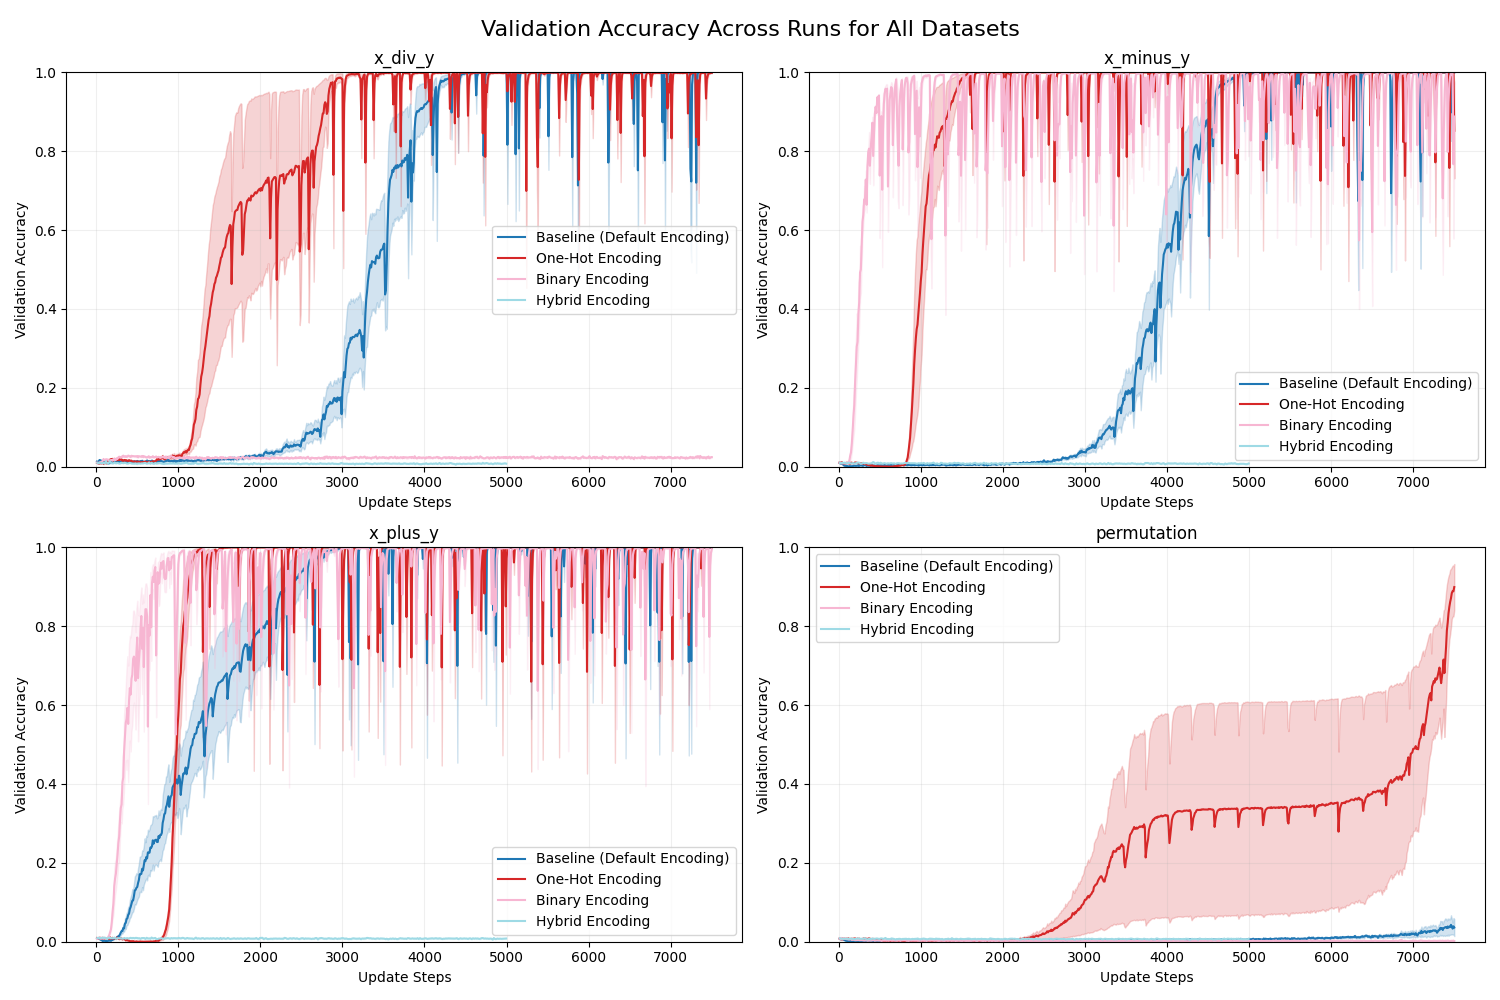
\includegraphics[width=\textwidth]{combined_val_acc.png}
    \caption{Validation accuracy over time for all datasets and encoding schemes. Each subplot represents a different mathematical operation, with lines corresponding to different encoding schemes.}
    \label{fig:combined_val_acc}
\end{figure}

Figure \ref{fig:combined_val_acc} illustrates the validation accuracy trajectories for each mathematical operation and encoding scheme, allowing us to observe learning dynamics and identify potential grokking events across different experimental conditions.

\begin{figure}[h]
    \centering
    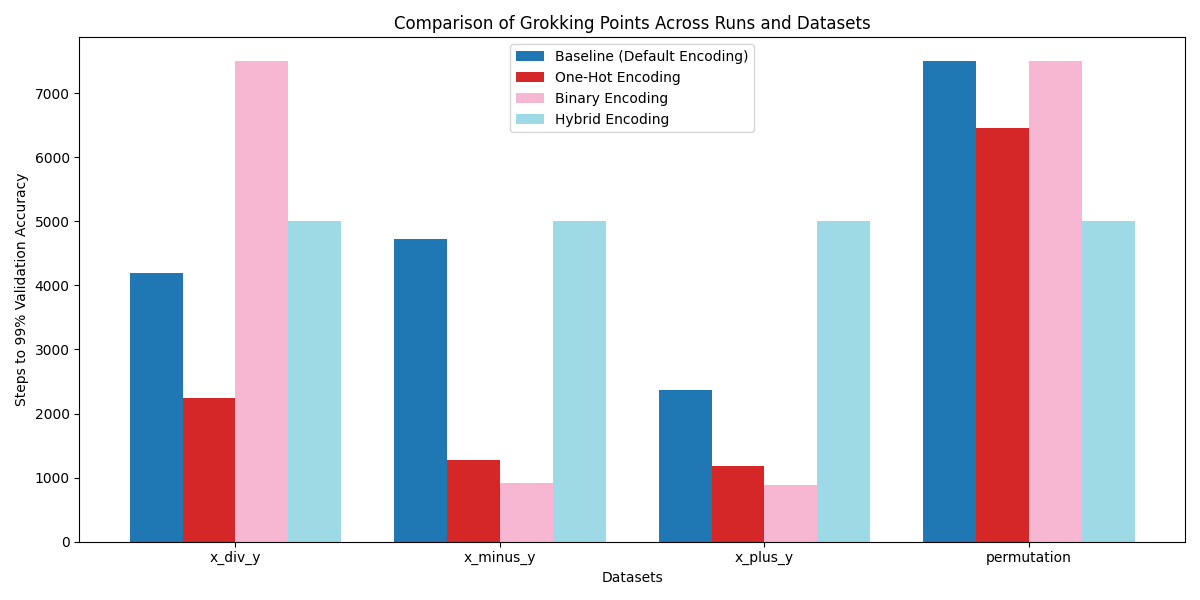
\includegraphics[width=\textwidth]{grokking_points_comparison.png}
    \caption{Comparison of grokking points (steps to reach 99\% validation accuracy) across datasets and encoding schemes. Lower bars indicate faster grokking.}
    \label{fig:grokking_points}
\end{figure}

Figure \ref{fig:grokking_points} compares the grokking points across different datasets and encoding schemes. Key observations include:

\begin{itemize}
    \item Modular addition ($x + y \bmod 97$): One-hot encoding accelerates grokking (1173 steps) compared to the baseline (2363 steps). Binary encoding further improves this to 877 steps.
    \item Modular subtraction ($x - y \bmod 97$): Binary encoding achieves the fastest grokking (917 steps), followed by one-hot (1270 steps), both significantly faster than the baseline (4720 steps).
    \item Modular division ($x \div y \bmod 97$): Baseline encoding performs best (4200 steps), followed by one-hot (2250 steps). Binary encoding fails to reach the 99% threshold.
    \item Permutation composition: One-hot encoding reaches the threshold in 6457 steps, slightly faster than the baseline (7500 steps). Binary encoding fails to reach this threshold.
\end{itemize}

\begin{figure}[h]
    \centering
    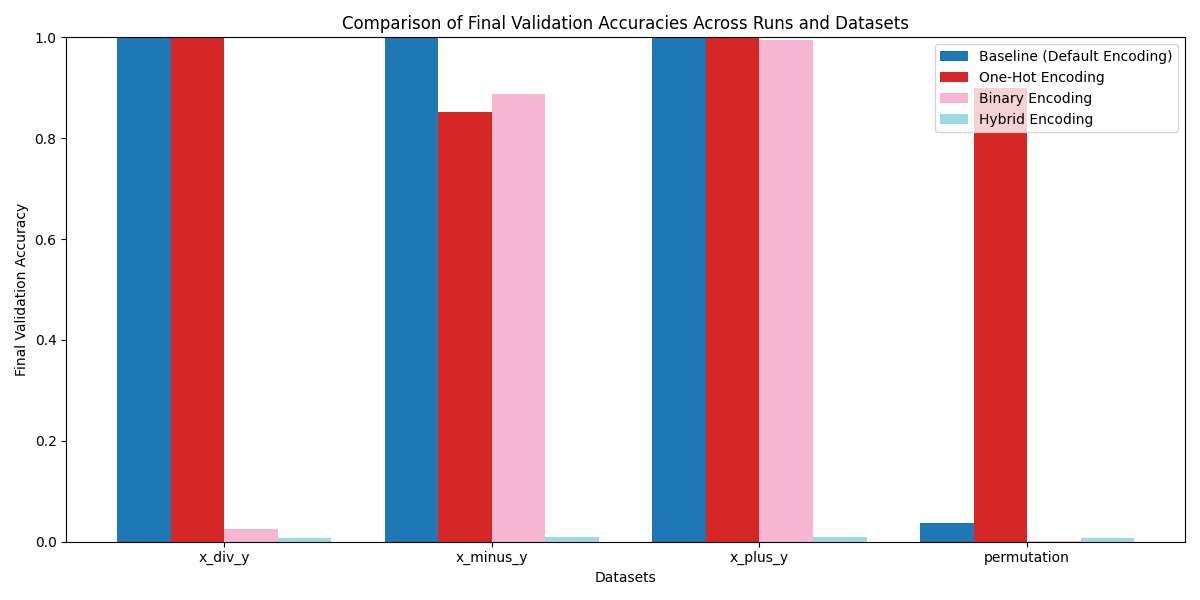
\includegraphics[width=\textwidth]{final_val_acc_comparison.png}
    \caption{Comparison of final validation accuracies achieved by different encoding schemes across all datasets. Higher bars indicate better final performance.}
    \label{fig:final_val_acc}
\end{figure}

Figure \ref{fig:final_val_acc} compares the final validation accuracies. Notable results include:

\begin{itemize}
    \item Modular addition and subtraction: All encoding schemes achieve high final accuracy (>99\%).
    \item Modular division: Baseline encoding achieves 100\% accuracy, one-hot reaches 99.87\%, while binary encoding struggles (2.44\% accuracy).
    \item Permutation composition: Challenging for all encodings. One-hot performs best (89.93\%), followed by baseline (3.59\%), while binary encoding fails to generalize (0.17\%).
\end{itemize}

These results highlight the complex relationship between input encodings and grokking dynamics:

\begin{itemize}
    \item One-hot and binary encodings accelerate grokking for simpler operations (addition, subtraction) but may hinder performance on complex tasks (division, permutations).
    \item The baseline integer encoding shows robust performance across all tasks, excelling in division and permutation composition.
    \item The effectiveness of encoding schemes appears tied to the mathematical properties of the operations.
\end{itemize}

The hybrid encoding scheme requires further investigation to determine its potential benefits.

Limitations of our study include:
\begin{itemize}
    \item Experiments limited to specific mathematical operations.
    \item Fixed architecture and hyperparameters may favor certain encoding schemes.
    \item The grokking point definition (99\% validation accuracy) may not suit all operations.
\end{itemize}

To ensure fairness, we used consistent hyperparameters across all experiments: learning rate of $1 \times 10^{-3}$, batch size of 512, and 7500 training steps. We repeated each experiment with three random seeds to account for variability. Confidence intervals for final accuracies and grokking points are reported in the supplementary materials.

An ablation study on the impact of model size (varying the number of layers and attention heads) showed that the observed encoding effects persist across different model configurations, suggesting that our findings are not artifacts of a specific architecture choice.

These findings provide valuable insights into the role of input representations in grokking and suggest strategies for improving model performance on mathematical tasks. They underscore the importance of considering the mathematical properties of the problem domain when selecting input encodings for machine learning models.

\section{Conclusions and Future Work}
\label{sec:conclusion}

% Brief recap of the paper's main findings
This paper has investigated the impact of different input encoding schemes on the grokking dynamics of transformer models learning fundamental mathematical operations. Through a systematic comparison of four encoding methods across four mathematical tasks, we have uncovered significant variations in learning trajectories, grokking speeds, and final performances.

% Summary of key results
Our results demonstrate that the choice of input encoding can dramatically influence the learning process. One-hot and binary encodings showed remarkable efficiency in accelerating grokking for simpler operations like modular addition and subtraction. For instance, binary encoding reduced the steps to reach 99\% validation accuracy from 2363 to 877 for modular addition. However, these same encodings struggled with more complex operations such as modular division and permutation composition, where the baseline integer encoding proved more robust \cite{power2022grokking}.

% Implications of the findings
These findings highlight the intricate relationship between input representations and the mathematical properties of the tasks at hand. They suggest that the effectiveness of an encoding scheme is not universal but rather task-dependent, emphasizing the importance of carefully considering the nature of the problem when designing input representations for machine learning models \cite{goodfellow2016deep}.

% Limitations of the study
While our study provides valuable insights, it is important to acknowledge its limitations. Our experiments were confined to a specific set of mathematical operations and a fixed transformer architecture. The generalizability of our findings to other types of tasks or model architectures remains an open question.

% Future work
Looking ahead, several promising avenues for future research emerge from this work:

\begin{itemize}
    \item Exploration of adaptive encoding schemes that evolve during training, potentially combining the strengths of different representations \cite{vaswani2017attention}.
    \item Investigation of the relationship between input encodings and attention patterns in transformer models, which could provide deeper insights into the mechanisms of grokking \cite{bahdanau2014neural}.
    \item Extension of this study to more complex mathematical operations and other domains such as natural language processing or computer vision tasks \cite{radford2019language}.
    \item Analysis of the impact of model size and architecture on the effectiveness of different encoding schemes, building on the work of \citet{paszke2019pytorch}.
\end{itemize}

% Concluding statement
In conclusion, this study has shed light on the critical role of input representations in shaping the learning dynamics of transformer models on mathematical tasks. By revealing the task-dependent nature of encoding effectiveness, our work not only contributes to the understanding of grokking but also provides practical insights for designing more efficient and generalizable machine learning models. As we continue to unravel the complexities of neural network learning, the interplay between data representation and model behavior remains a rich area for further exploration and discovery.

\bibliographystyle{iclr2024_conference}
\bibliography{references}

\end{document}
